\documentclass{article}

\usepackage{fancyhdr}
\usepackage[german]{babel}
\usepackage{geometry}
\usepackage{fontspec}
\usepackage{graphicx}
\usepackage{listings}
\usepackage{float}

\pagestyle{fancy}
\linespread{1.25}
\setmainfont{Liberation Sans}
\setlength{\parindent}{0cm}
\graphicspath{ {./images/} }

\begin{document}
	
	\fancyfoot{}
	\fancyhead{}
	\fancyhead[c]{Wacky Whoooo Pizza Hist Delivery Adventure}
	\fancyhead[r]{\today}
	\fancyhead[l]{Marcel Frank Kucera}
	\fancyfoot[c]{\thepage}
	
	\thispagestyle{empty}
	\begin{centering}
		\centering
		{\Large Dokumentation im Fach Praktische Informatik}\\
		Schuljahr 2019/202\\
		\vspace{3cm}
		{\Large Theodor-Litt-Schule Gießen}\\
		\vspace{3cm}
		{\Huge \textbf{Wacky Whoooo Pizza Hist Delivery Adventure}}\\
		\vspace{0.5cm}
		{\Large Die Entwicklung eines objektorientiertem Spiels\\in der Godot Engine}\\
		\vspace{3cm}
		{\Large von\\Marcel Frank Kucera}\\
		\vspace{2cm}
		\today
		\vfill
		\hfill \underline{vorgelegt bei:}\\
		\hfill Herr Magdeburg
	\end{centering}

	\newpage
	\tableofcontents
	\thispagestyle{empty}

	\newpage
	\pagenumbering{arabic}
	
	\section{Einleitung}
	
	Zuerst wird die Projektplanung vorgestellt. Darin wird die Produktskizze gezeigt und das Konzept des Spiels vorgestellt. Dazu kommen einige Prototypen dazu, welche zeigen, wie das Spiel hätte aussehen können. Danach folgt der Versionierungsplan des Projekts, welcher darstellt, welche Features in das Spiel, bei der jeweiligen Versionsnummer implementiert werden sollten. Daraufhin wird der Entwurf des Spiels dargestellt, dort werden einige Klassendiagramme von den Klassen des Spiels vorgestellt und eine Methode per Struktogramm genauer beschrieben. Zuletzt wird die Durchführung dieser Idee gezeigt. Dazu werden einige Ausschnitte aus dem Quelltext mithilfe von Kommentaren genauer beschrieben und Screenshots des finalen Produkts gezeigt.\\
	
	Ich habe mich bei diesem Projekt für die Godot Engine anstatt Greenfoot entschieden, da ich mithilfe dieses Projekts die Grundlagen für die Spielprogrammierung lernen wollte und ich der Meinung bin, dass Greenfoot nur wenige Möglichkeiten hinaus den grundlegenden Funktionen bietet und somit nicht für die Spielentwicklung geeignet ist. Des Weiteren hasse ich Greenfoot. Ich bin auf die Godot Engine gekommen, da diese oft als FOSS Alternative für die, als Einsteiger freundlich bekannte, Unity Engine genannt wird.

	\section{Planung}
	\subsection{Produktskizze}
	
	\textbf{Name:}\\
	Wacky Whoooo Pizza Hist Delivery Adventure\\
	\textbf{Genre:}\\
	Pizzalieferdienst Simulator / Topdown-Shooter\\
	\textbf{Aufgaben und Vorgehen des Spielers:}\\
	Der Spieler ist damit beauftragt Pizzen an bestimmte Orte auszuliefern. Jedoch wird er währenddessen von feindlichen Kugelfischen verfolgt, welche versuchen, ihn an seiner Mission, die Pizzen auszuliefern, zu hindern. Er kann die Gegner aufhalten, indem er diese mit Pizza abwirft, bis sie die Verfolgung aufgeben und verschwinden. Er selbst  verliert, wenn die Gegner ihn so oft angegriffen haben, dass seine Leben auf 0 fallen. Die Struktur des Spieles besteht aus einem Endlosmodus, bei welchem der Spieler so lange Pizzen ausliefern muss, bis er von den Gegnern aufgehalten wird.
	
	\subsection{Prototypen}
	
	Diese Prototypen stellen die Konzepte verschiedene Zustände des Spieles, wie sie zu Beginne der Entwicklung geplant waren, dar. Das Aussehen dieser Zustände stand dabei nicht im Vordergrund, weshalb die Prototypen unschön aussehen. Da diese vor dem Beginn der Entwicklung des Spiels entstanden sind, kommt es vor, dass einige Funktionen, welche auf den Prototypen dargestellt werden, nicht im finalen Spiel enthalten sind.
	
	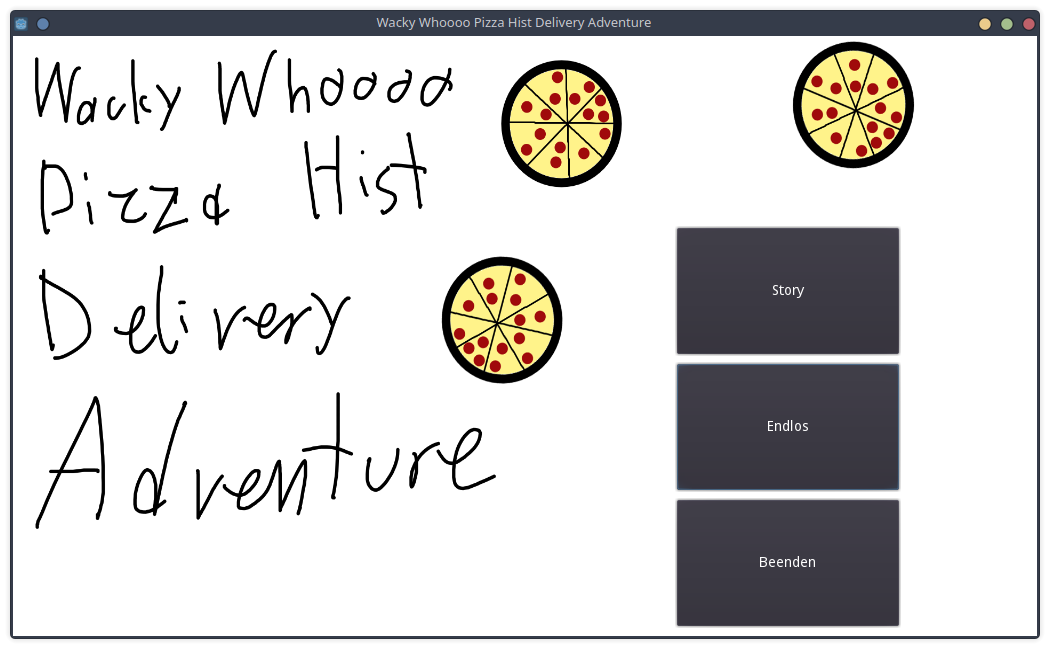
\includegraphics[width=\textwidth]{start.png}
	\textbf{Spielbeginn (Titelbildschirm):}
	Man hat drei Auswahlmöglichkeiten:
	\begin{itemize}
		\item Story(Startet Storymodus)
		\item Endlos (Startet Endlosmodus)
		\item Beenden (Beendet das Spiel)
	\end{itemize}
	Hier ist zu beachten, dass der Storymodus, auf welchen in diesem Prototyp hingewiesen wird, nicht im finalen Spiel enthalten ist.\\
	
	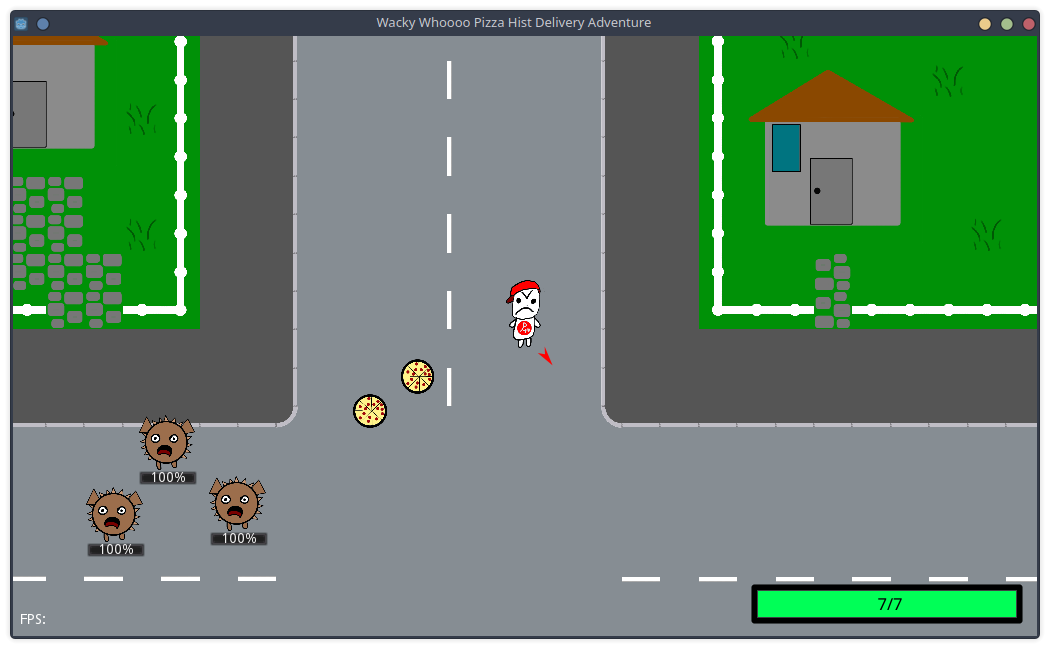
\includegraphics[width=\textwidth]{ingame.png}
	\textbf{Ingame:}
	Hier ist ein Bild aus dem Endlosmodus.
	Zusehen ist
	\begin{itemize}
		\item Spieler Charakter
		\begin{itemize}
			\item Die von ihm geworfenen Pizzas
		\end{itemize}
		\item Gegner
		\item Lebens Anzeige (7/7)
		\item Missionsanzeige (Roter Pfeil bei Spieler)
	\end{itemize}
	Der Spieler wird mit WASD gesteuert und die Pizzen mit Linksklick in Richtung der Maus geworfen.
	Man kann unter den Gegnern ihre Ausdauer sehen. Sollte diese auf null fallen werden sie sich zurückziehen und so nicht mehr den Spieler behindern.
	Der rote Pfeil zeigt an wo der Missionsort des Spielers liegt.
	
	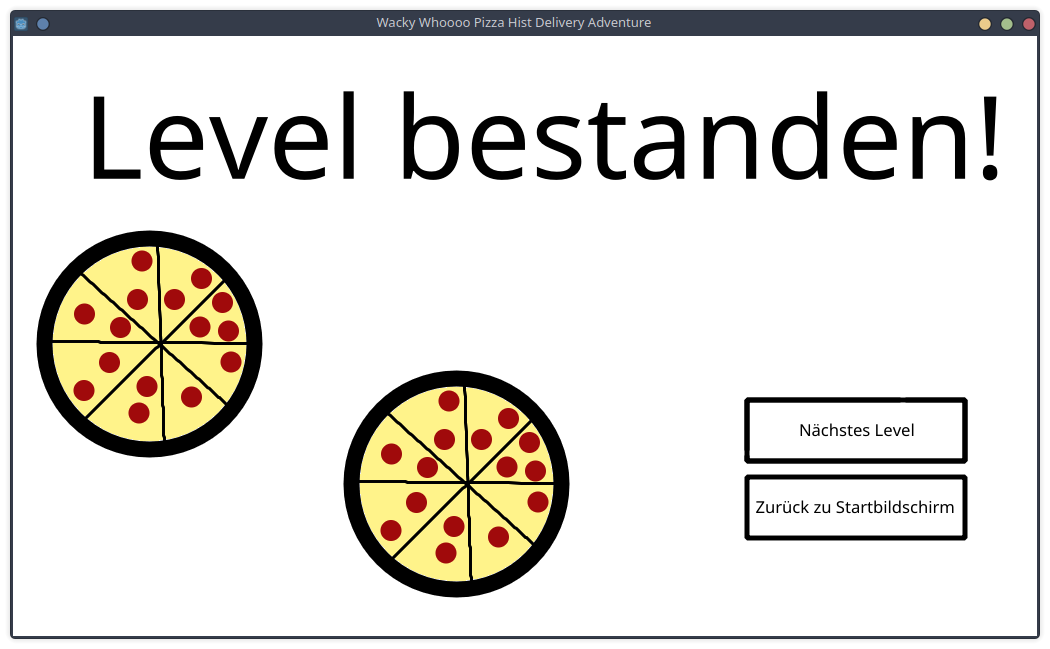
\includegraphics[width=\textwidth]{end.png}
	\textbf{Missions Ende:}
	Im Rahmen des Storymodus war auch ein „Mission erledigt“ Bildschirm geplant. Dieser wurde jedoch überflüssig, da der Storymodus entfernt wurde.
	
	\newpage
	\subsection{Versionierung}
	\begin{table}[h]
		\begin{tabular}{|l|l|}
			\hline
			\textbf{Version} & \multicolumn{1}{c|}{\textbf{Funktion}}  \\ \hline
			0.1              & Spieler Akteur mit Bewegung            \\ \hline
			0.2              & Test Spielwelt                         \\ \hline
			0.3              & Spieler Pizzen werfen                  \\ \hline
			0.4              & Implementierung von Akteur Klasse      \\ \hline
			0.5              & Gegner Akteur mit einfacher Verfolgung \\ \hline
			0.5.5            & Gegner navigieren um Hindernisse       \\ \hline
			0.5.7            & Gegner erscheinen um den Spieler herum \\ \hline
			0.6              & Lebenssystem für Spieler und Gegner    \\ \hline
			0.7              & Animationen für Spieler und Gegner     \\ \hline
			0.8              & Score und Highscore                    \\ \hline
			0.9              & Start- und Endbildschirm               \\ \hline
			0.10             & Finale Spielwelt                       \\ \hline
			0.11             & Upgrade Shop und Geld                  \\ \hline
			1.0              & Abgabebereit                           \\ \hline
			1.1              & Gegnervariation                        \\ \hline
		\end{tabular}
	\end{table}
	
	Die Abgegebene Version ist die Version 1.0

	\section{Entwurf}
	\subsection{Klassendiagramme}
	
	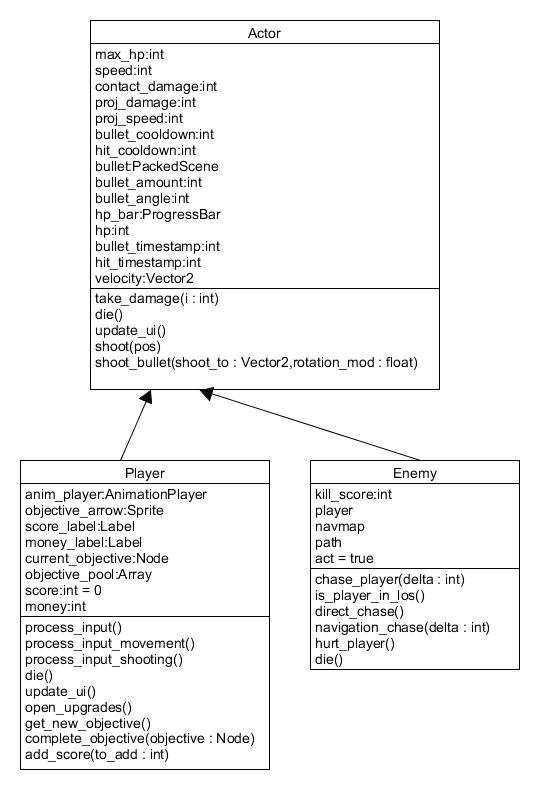
\includegraphics[height=\linewidth]{klassendiagramm1.jpg}\\
	In diesem Klassendiagramm sieht man den Aufbau der Player und Enemy Klasse. Diese beiden Klassen erben von der Akteur-Klasse. Die Akteur-Klasse stellt die notwendigen Variablen und Methoden zu Verfügung, welche benötigt werden, damit das Objekt sich in der Spielwelt bewegen kann, es Schaden bekommen und Sterben kann, seine Lebensanzeige aktualisieren kann und es Projektile verschießen kann. Die Logik für die Projektile stehen in der Akteur-Klasse, obwohl diese nur von dem Spieler verwendet werden, da in einer späteren Version geplant ist, dass einige Gegner die Funktion haben auch auf den Spieler zu schießen.\\
	
	
	Die Player-Klasse hat zusätzlich die Eingabe Verarbeitung, womit man der Spieler sich in der Spielwelt bewegen und schießen kann. Zudem enthält diese Klasse auch die Scorelogik und die Missionslogik, womit der Spieler Pizzen für extra Punkte und Heilung ausliefern kann. Des Weiteren wird die Methode „die()“ aus der Akteur-Klasse überschrieben, damit das Spielerobjekt sich nicht selbst entfernt, sondern zu dem Verlieren-Bildschirm wechselt.\\
	
	Die Enemy-Klasse erweitert die Akteur-Klasse nur, indem sie die Logik zu der Verfolgung und Interaktion mit dem Spieler hinzufügt.\\
	
	\begin{centering}
		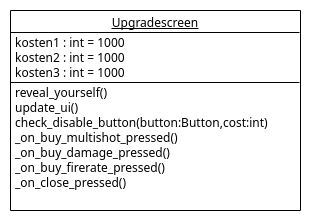
\includegraphics[width=7cm]{klassendiagramm2.png}\\
	\end{centering}
	In diesem Klassendiagramm wird der Upgrade-Bildschirm dargestellt. Die Variablen stellen die Verschiedenen Preise der Upgrades dar. Diese Klasse enthält Methoden, um die Benutzeroberfläche zu aktualisieren und die Upgrades zu kaufen.
	
	\subsection{Struktogramm einer Methode}

	\begin{centering}
		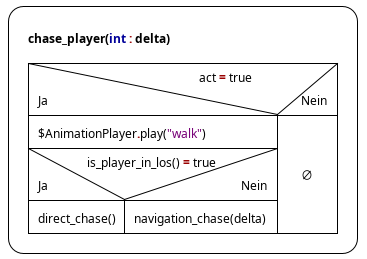
\includegraphics[width=7cm]{chase.png}\\
	\end{centering}
	Die Methode chase\_player() verursacht, dass der Gegner den Spieler verfolgt. Dazu überprüft diese zuerst, ob der Gegner sich bewegen soll. Danach prüft es, ob der Gegner eine direkte Sichtlinie zum Spieler hat. Ist dies der Fall wird die Methode direct\_chase() aufgerufen, um den Spieler ohne Wegfindung und die Verfolgung natürlicher aussieht. Ist dies jedoch nicht der Fall, navigiert der Gegner mit der Methode navigation\_chase() zum Spieler, während er Hindernisse vermeidet.\\
	
	\begin{centering}
		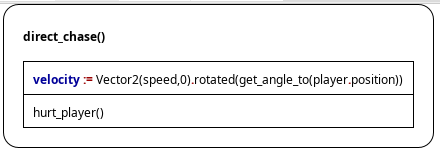
\includegraphics[width=7cm]{direct.png}\\
	\end{centering}
	Die Methode direct\_chase() bewegt den Gegner ohne Wegfindung direkt zum Spieler hin. Dazu setzt diese den Geschwindigkeitsvektor auf die Bewegungsgeschwindigkeit und rotiert diesen zum Spieler hin. Danach verursacht es Schaden am Spieler, sollte der Gegner in diesem stehen.\\
	
	\begin{centering}
		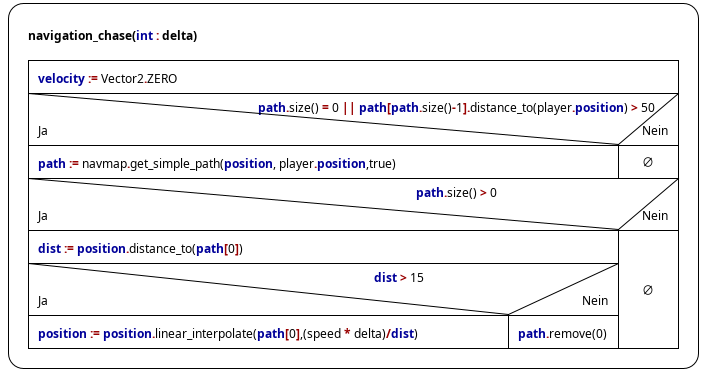
\includegraphics[width=12cm]{nav.png}\\
	\end{centering}
	Die Methode navigation\_chase() sucht einen Weg zum Spieler und bewegt dann den Gegner entlang diesem Weg. Dazu wird geprüft, ob es schon ein Weg berechnet wurde und, ob dieser noch aktuell ist. Sollte dies nicht der Fall sein, wird ein neuer Weg berechnet. Danach wird der Weg geprüft, damit keine Fehler entstehen und der Gegner wird entlang des Weges bewegt.

	\section{Durchführung}
	\subsection{Kommentierter Quelltext}
	
	Dies ist die gesamte Player-Klasse, welche die Logik für Eingaben, Missionen, Score und Benutzeroberfäche enthält
	
	\begin{verbatim}
	# Spieler erbt von der Klasse Actor
extends Actor

# Kinder Nodes für Benutzer Oberfläche
var anim_player
var objective_arrow
var score_label
var money_label

# Variablen zu Missionen, Score und Geld
var current_objective:Node
var objective_pool:Array #Enthält alle Abliefer Punkte
var score:int = 0
var money:int

# Initialisiert alle wichtige Variablen:
func _ready():
    # 1. Objekte für Benutzeroberfläche
    hp_bar = $UI/MenuBG/MarginContainer/VBoxContainer/HP_Bar
    anim_player = $Sprite/AnimationPlayer
    objective_arrow = $Sprite/Arrow
    score_label = $UI/MenuBG/MarginContainer/VBoxContainer/Score
    money_label = $UI/MenuBG/MarginContainer/VBoxContainer/Money
    
    gamestate.player = self # 2. Trägt Spiele in globale Variable ein
    gamestate.current_score = 0
    objective_pool = get_parent().get_objectives() #Läd alle Missionspunkte
    get_new_objective() #Sucht den ersten Missionspunkt aus

#Ruft alle Methoden auf, die die Eingabe des Spielers verarbeiten
func process_input():
    process_input_movement()
    process_input_shooting()

#Prüft auf Richtungseingaben und setzt dann die Geschwindigkeit des Spielers 
func process_input_movement():
    #Prüft auf eingaben
    velocity = Vector2()
    if Input.is_action_pressed('right'):
        velocity.x += 1
        $Sprite.flip_h = false
        $Sprite/Node2D.scale = Vector2(1,1)
    if Input.is_action_pressed('left'):
        velocity.x -= 1
        $Sprite.flip_h = true
        $Sprite/Node2D.scale = Vector2(-1,1)
    if Input.is_action_pressed('down'):
        velocity.y += 1
    if Input.is_action_pressed('up'):
        velocity.y -= 1
    
    #Spiele die angemessene Animation für die Geschwindigkeit
    if velocity == Vector2.ZERO:
        anim_player.play("Rest")
    else:
        anim_player.play("Walk")

    #Stellt sicher, dass die Bewegungsgeschwindigkeit immer gleich bleibt	
    velocity = velocity.normalized() * speed 

#Prüft, ob der Spieler schießt und ruft dann shoot() aus der Geerbten
#Klasse mit der Mausposition als Parameter auf
func process_input_shooting():
    if Input.is_action_pressed("shoot"):
        shoot(get_global_mouse_position())

#Wenn die Leben auf 0 fallen, wird der Score gespeichert
#und es wird zum Failscreen gewechselt
func die():
    gamestate.new_score(score)
    get_tree().change_scene("res://scenes/failscreen/FailScreen.tscn")

#Aktualisiert die Benutzeroberfläche
func update_ui():
    .update_ui() #Ruft Methode aus Actor-Klasse auf
    objective_arrow.look_at(current_objective.position)
    objective_arrow.rotation += deg2rad(90)
    score_label.text = "Score: " + str(score)
    money_label.text = "Money: " + str(money)

#Öffnet Upgrade-Bildschirm
func open_upgrades():
    $UI/Upgrades.reveal_yourself()

#Suchte wechselt den derzeitigen Missionspunkt zu einem neuen aus dem Pool
func get_new_objective():
    current_objective = objective_pool[int(rand_range(0,objective_pool.size()))]

#Wird aufgerufen, wenn ein Missionspunkt berührt wurde
func complete_objective(objective):
    if(objective == current_objective): #Prüft ob Missionspunkt der Aktive ist

        #Heilung
        hp += 1
        if (hp > max_hp):
            hp = max_hp
        
        add_score(500) #Fügt extra Score hinzu

        #Wenn der Missionpool leer ist, wird dieser wieder aufgefüllt
        if(objective_pool.size() == 1):
            objective_pool = get_parent().get_objectives()

        #Entfernt den Berührten Missionspunkt aus dem Missionspool 
        #und wählt eine neue Mission aus
        objective_pool.erase(current_objective) 
        get_new_objective()

#Fügt Score und so auch Geld hinzu
func add_score(to_add):
    score += to_add
    money += to_add

#Hauptschleife
#Wird bei zu jedem Frame ausgeführt
func _physics_process(_delta):
    process_input()
	\end{verbatim}
	\newpage
	
	\subsection{Screenshots}
	
			\begin{figure}[H]
				\begin{center}
					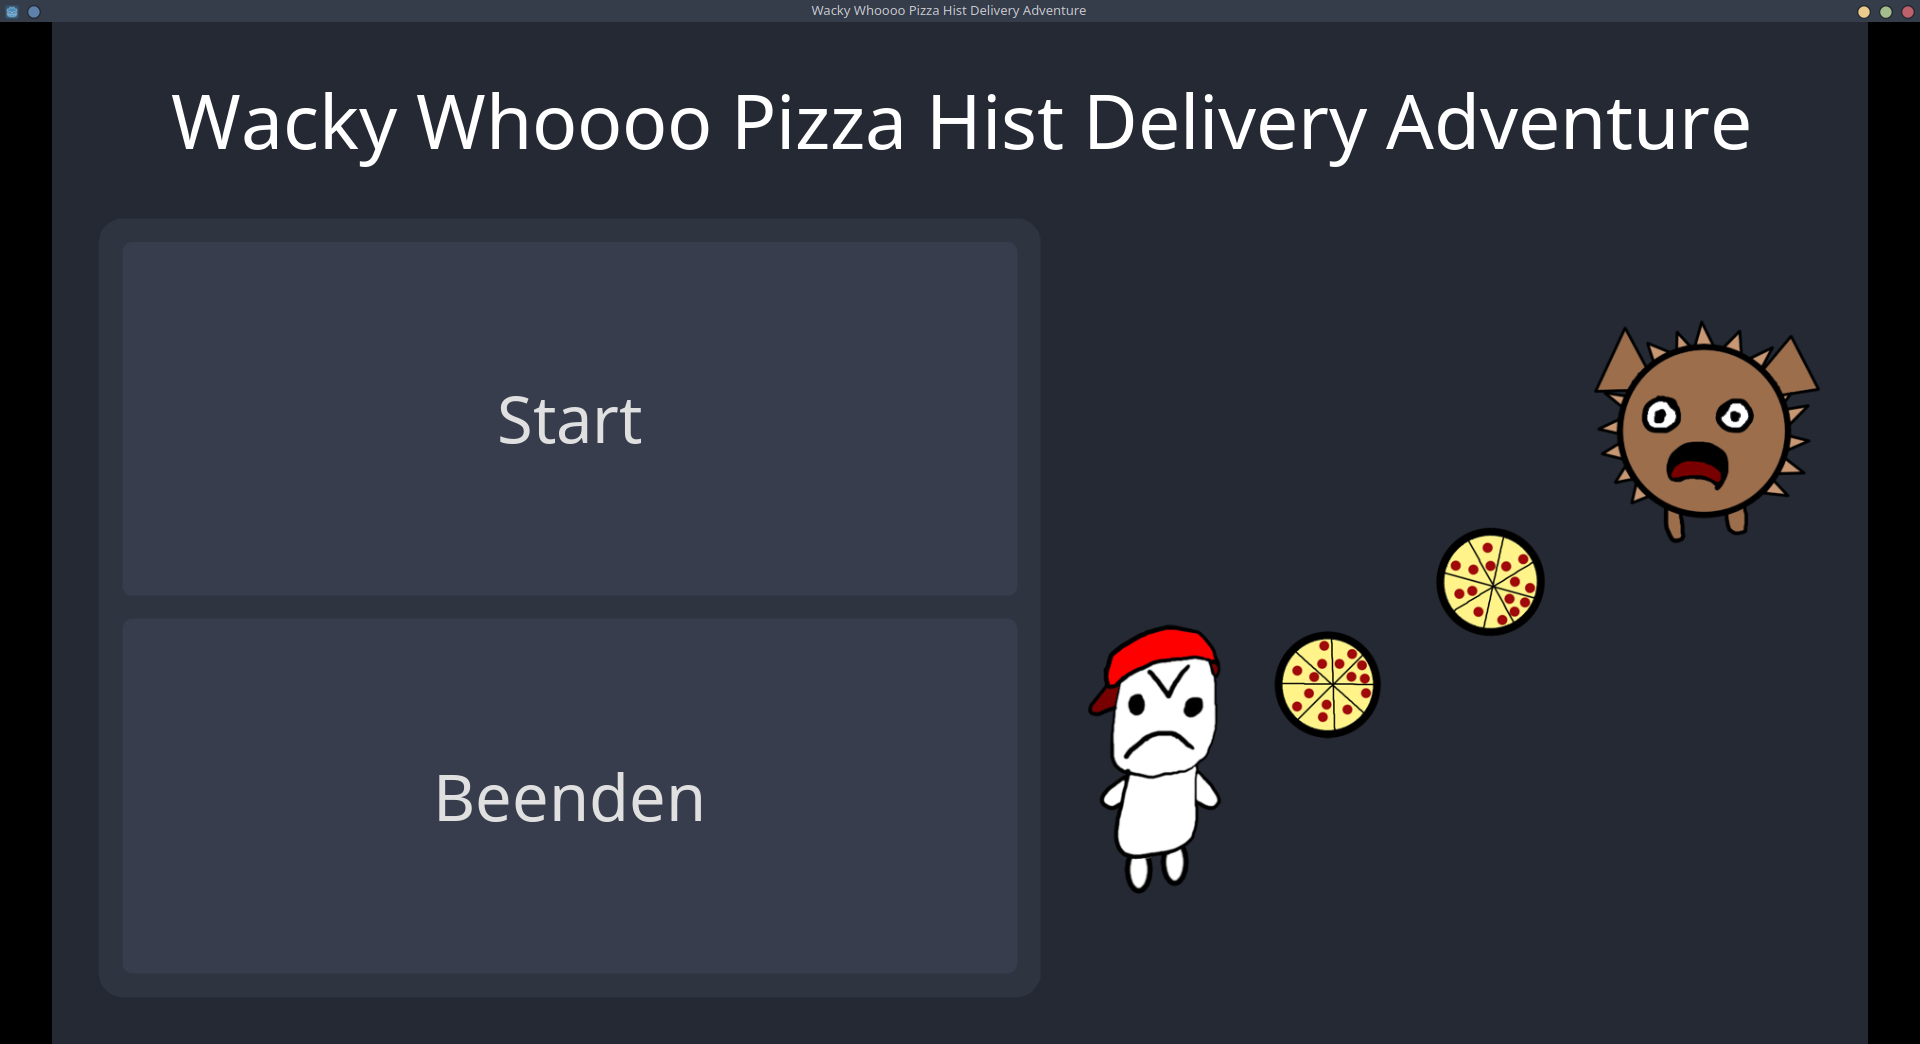
\includegraphics[width=0.8\textwidth]{start2.png}
				\end{center}
				\caption{Titelbildschirm}
			\end{figure}
			\begin{figure}[H]
				\begin{center}
					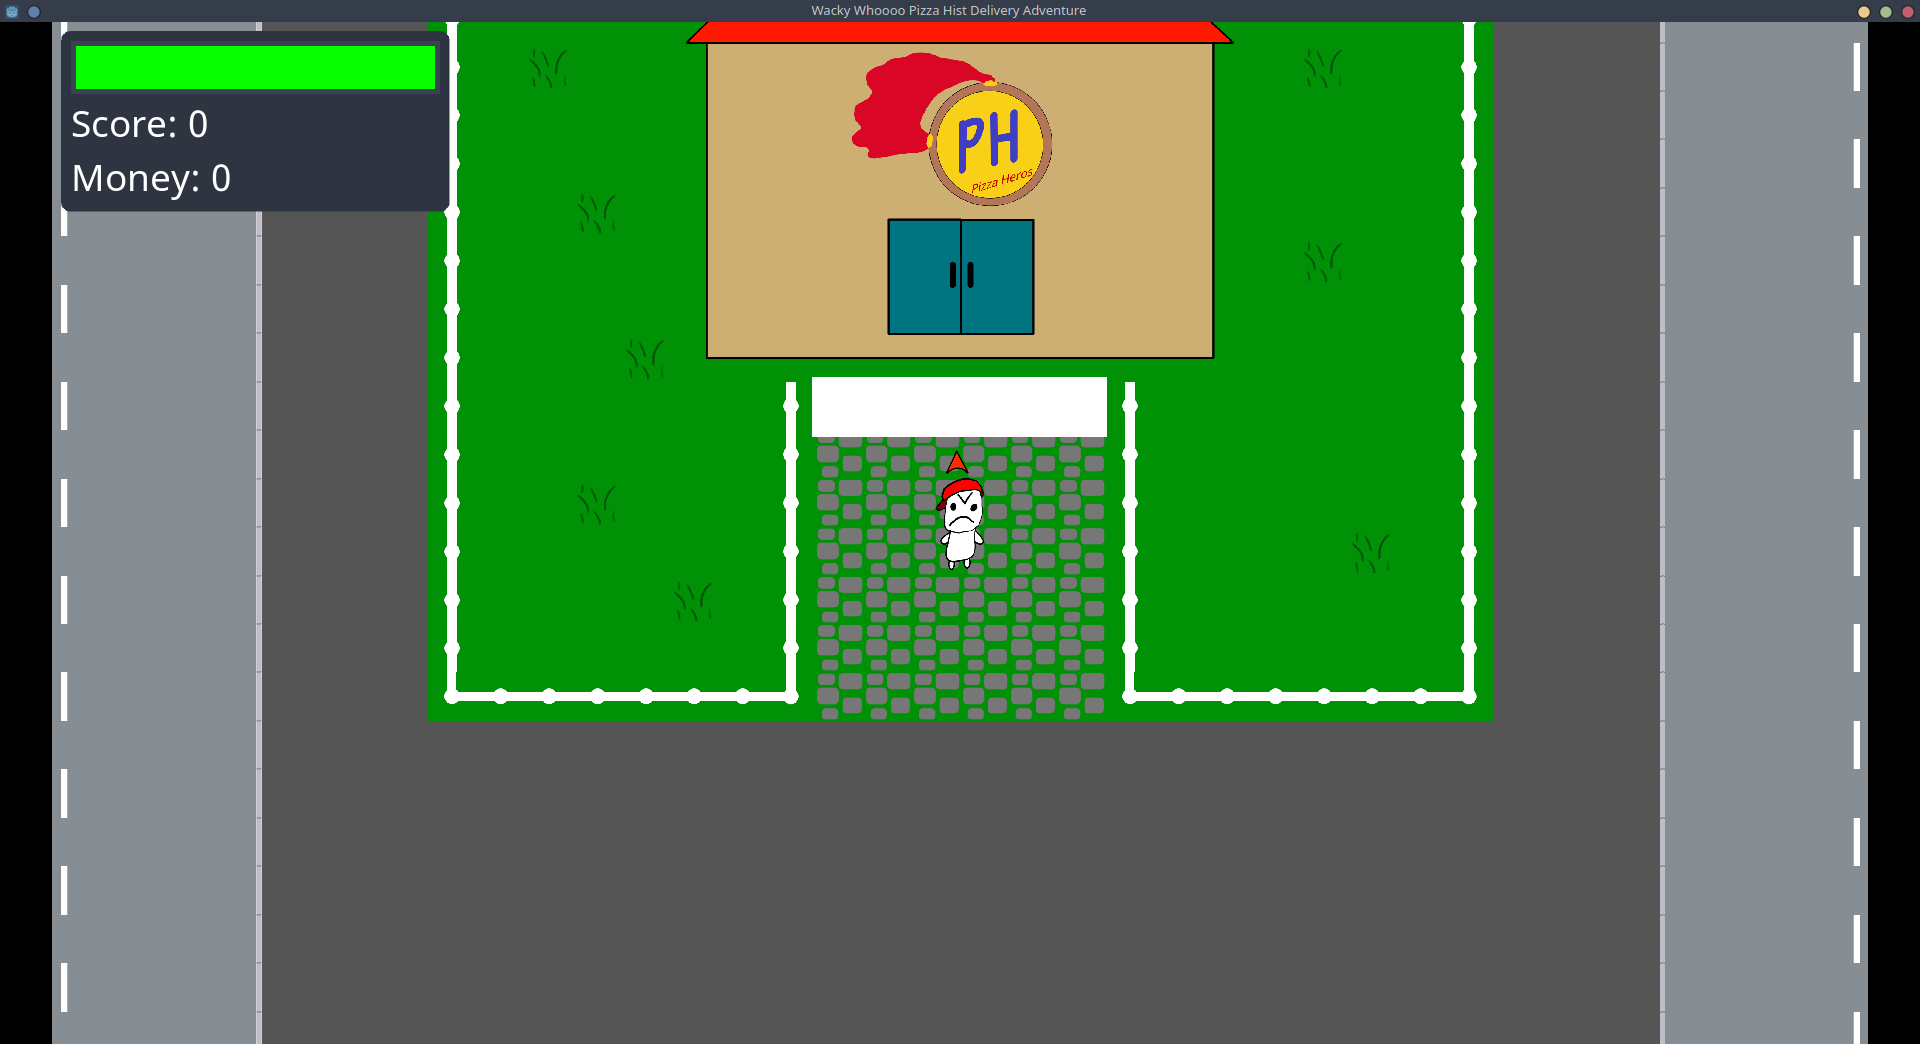
\includegraphics[width=0.8\textwidth]{spielbeginn.png}
				\end{center}
				\caption{Spielbeginn}
			\end{figure}
			\begin{figure}[H]
				\begin{center}
					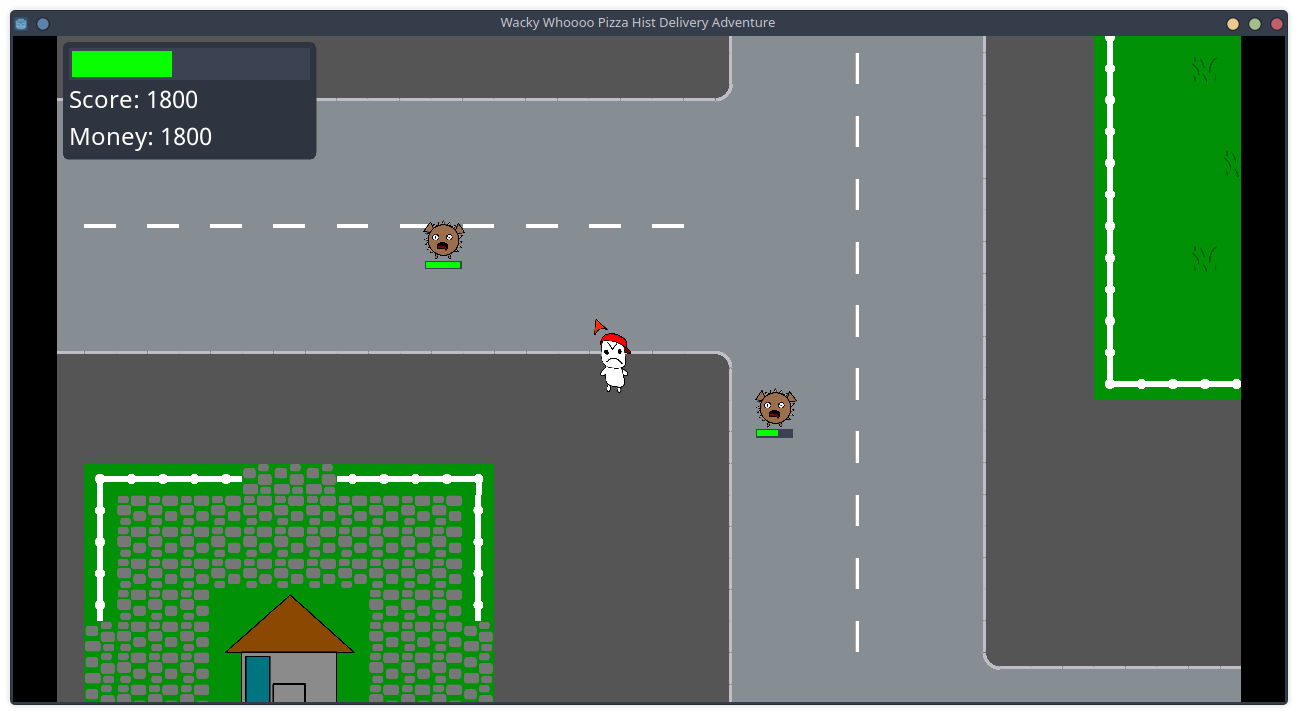
\includegraphics[width=0.8\textwidth]{ingame2.png}
				\end{center}
				\caption{Im Spiel}
			\end{figure}
			\begin{figure}[H]
				\begin{center}
					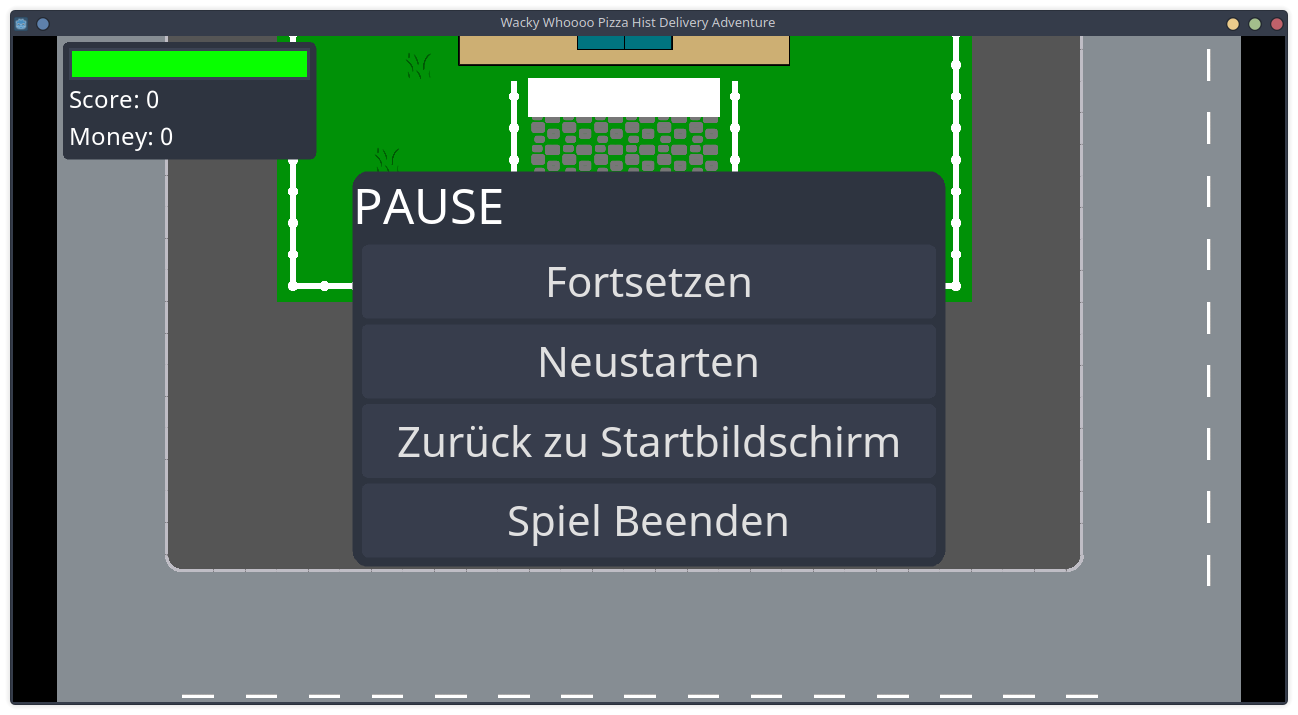
\includegraphics[width=0.8\textwidth]{pause.png}
				\end{center}
				\caption{Pausemenü}
			\end{figure}
			\begin{figure}[H]
				\begin{center}
					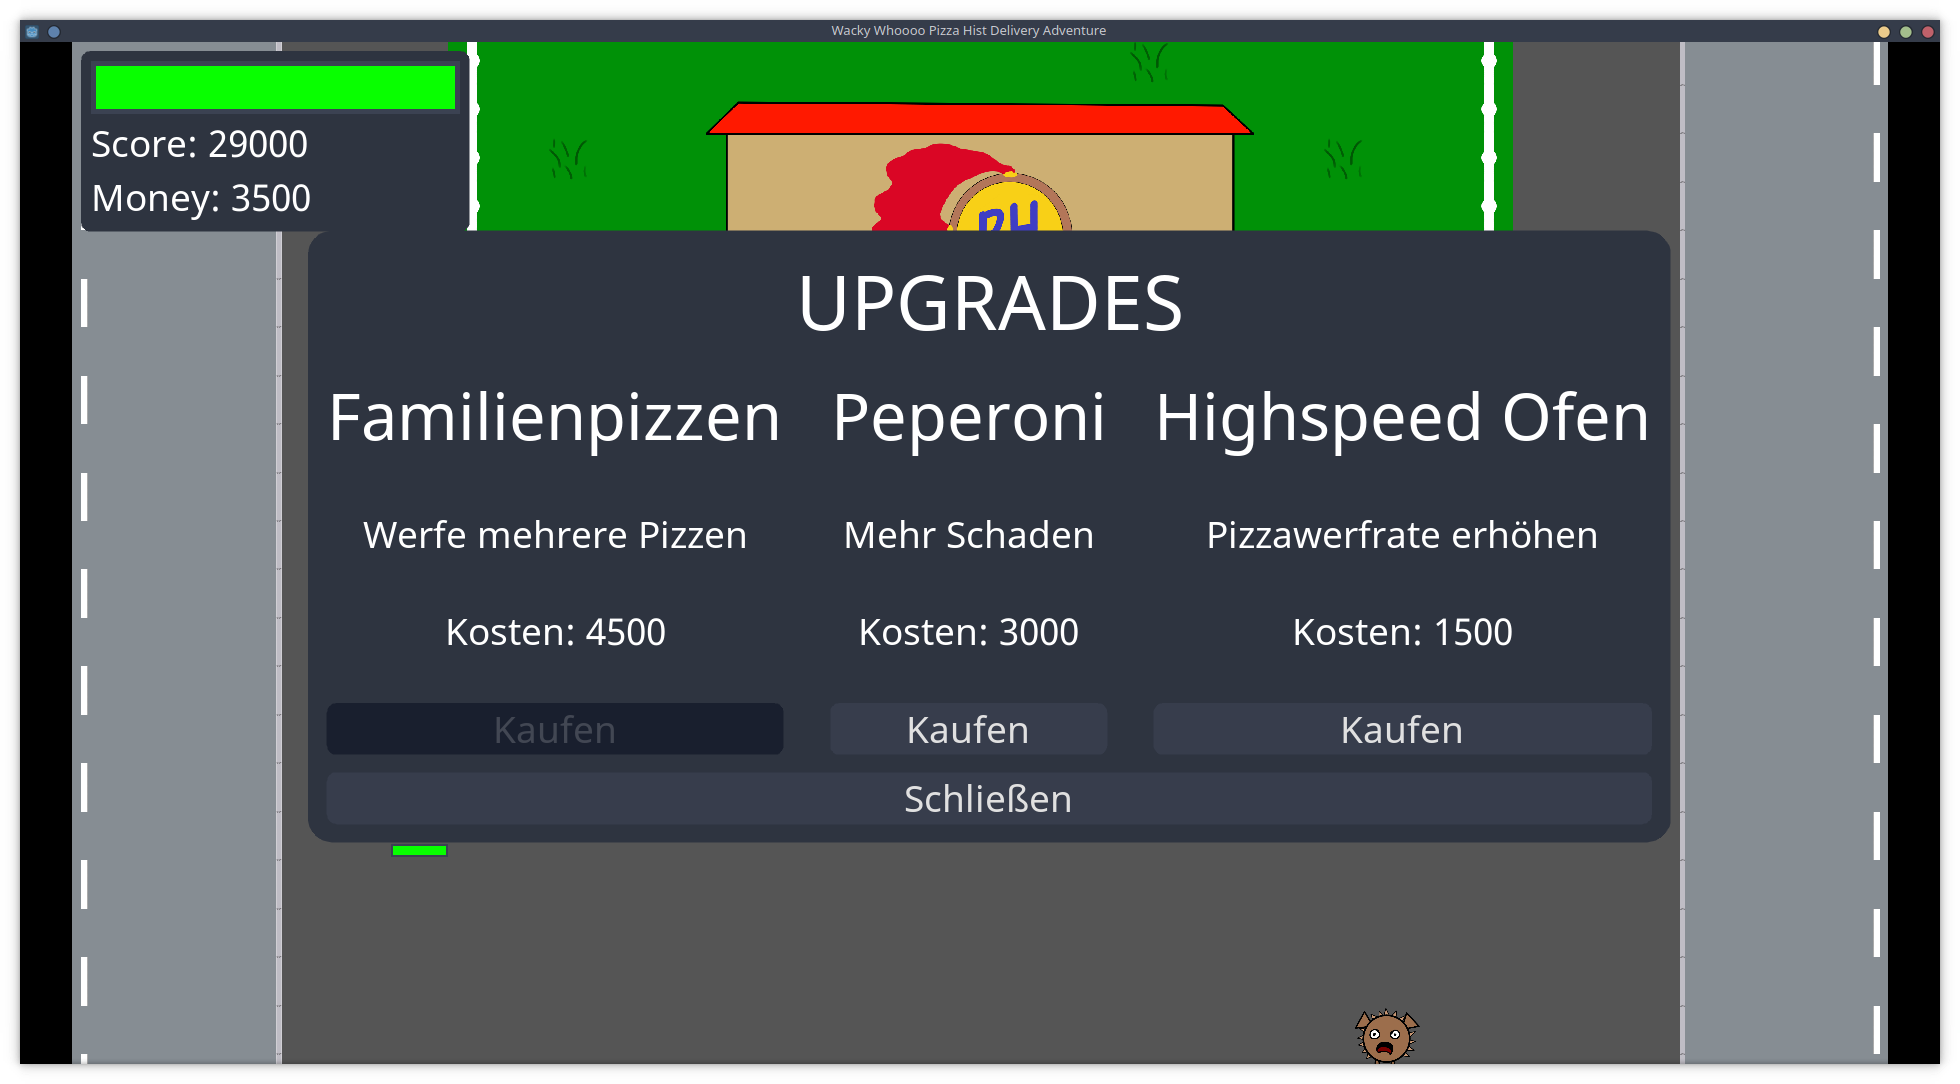
\includegraphics[width=0.8\textwidth]{upgrade.png}
				\end{center}
				\caption{Upgrade Menü}
			\end{figure}
			\begin{figure}[H]
				\begin{center}
					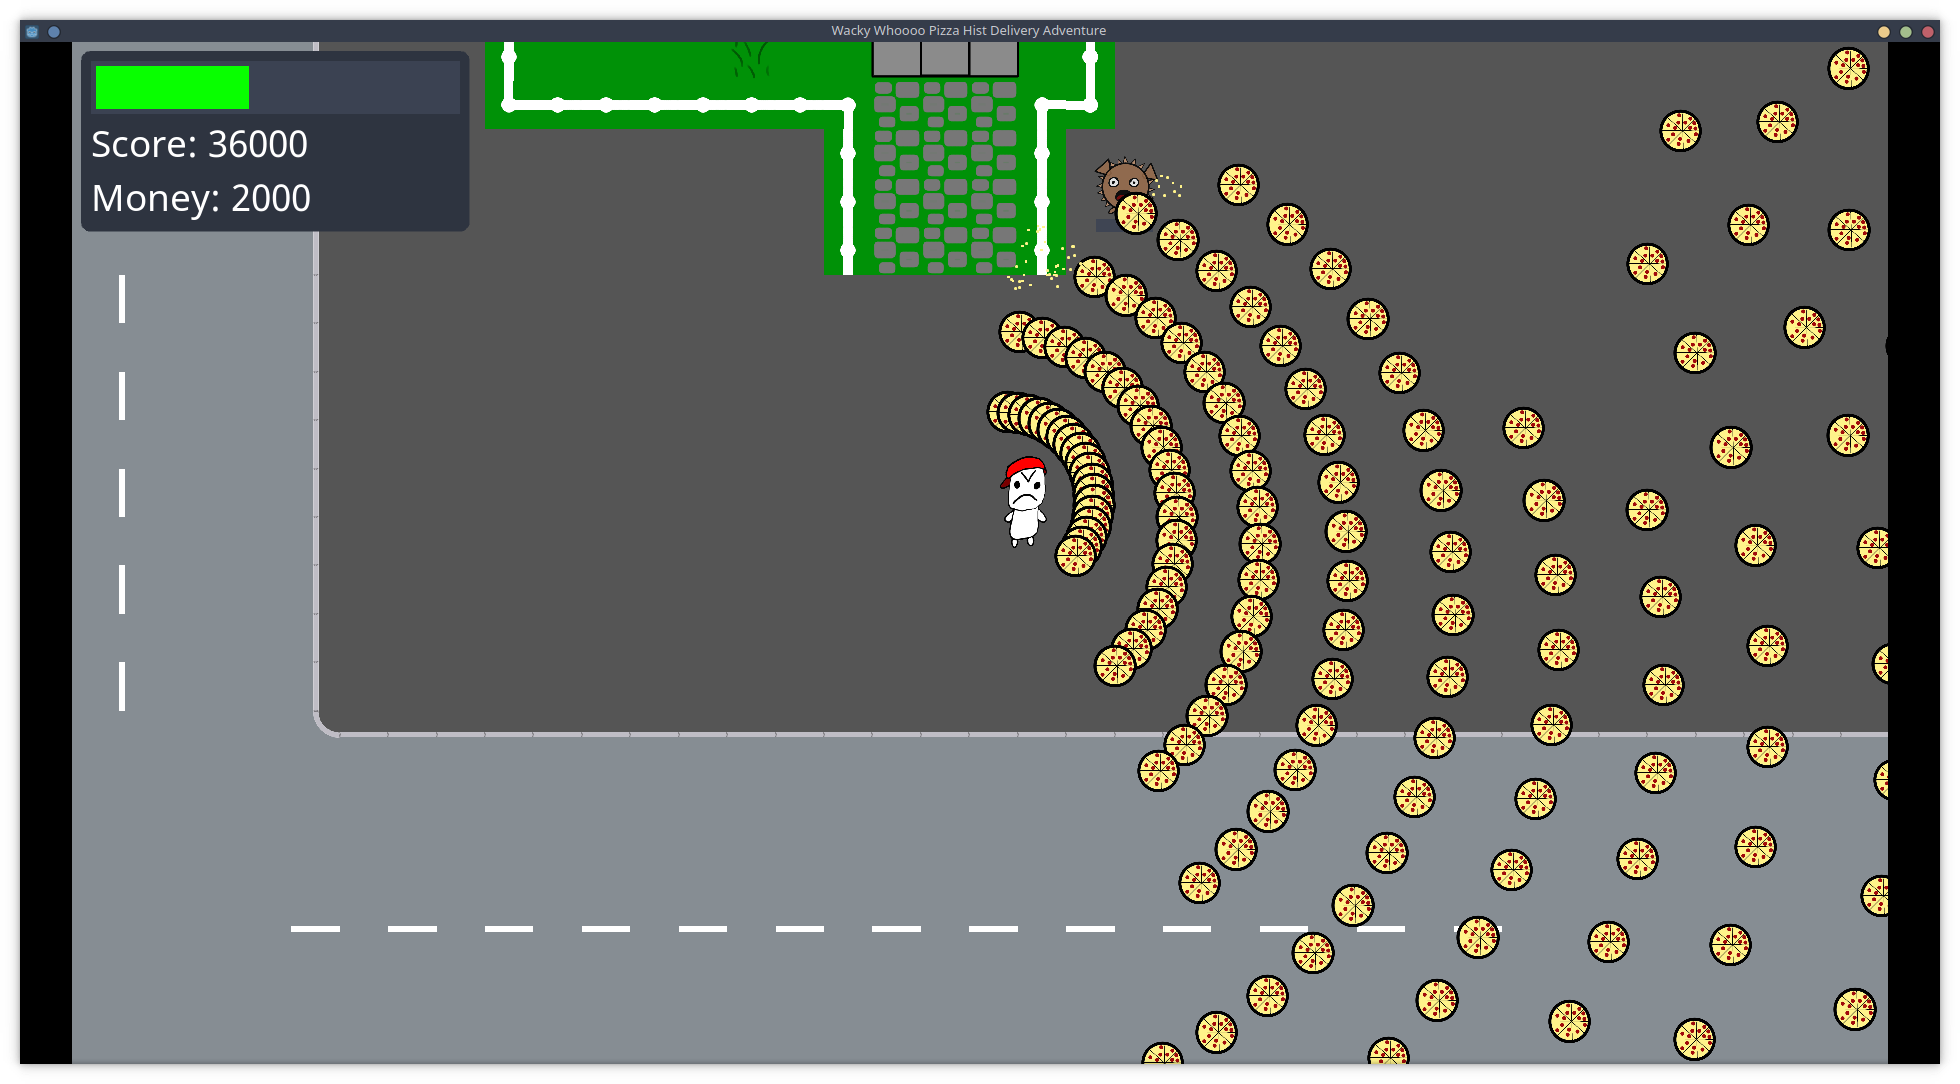
\includegraphics[width=0.8\textwidth]{lategame.png}
				\end{center}
				\caption{Späterer Spielverlauf}
			\end{figure}
			\begin{figure}[H]
				\begin{center}
					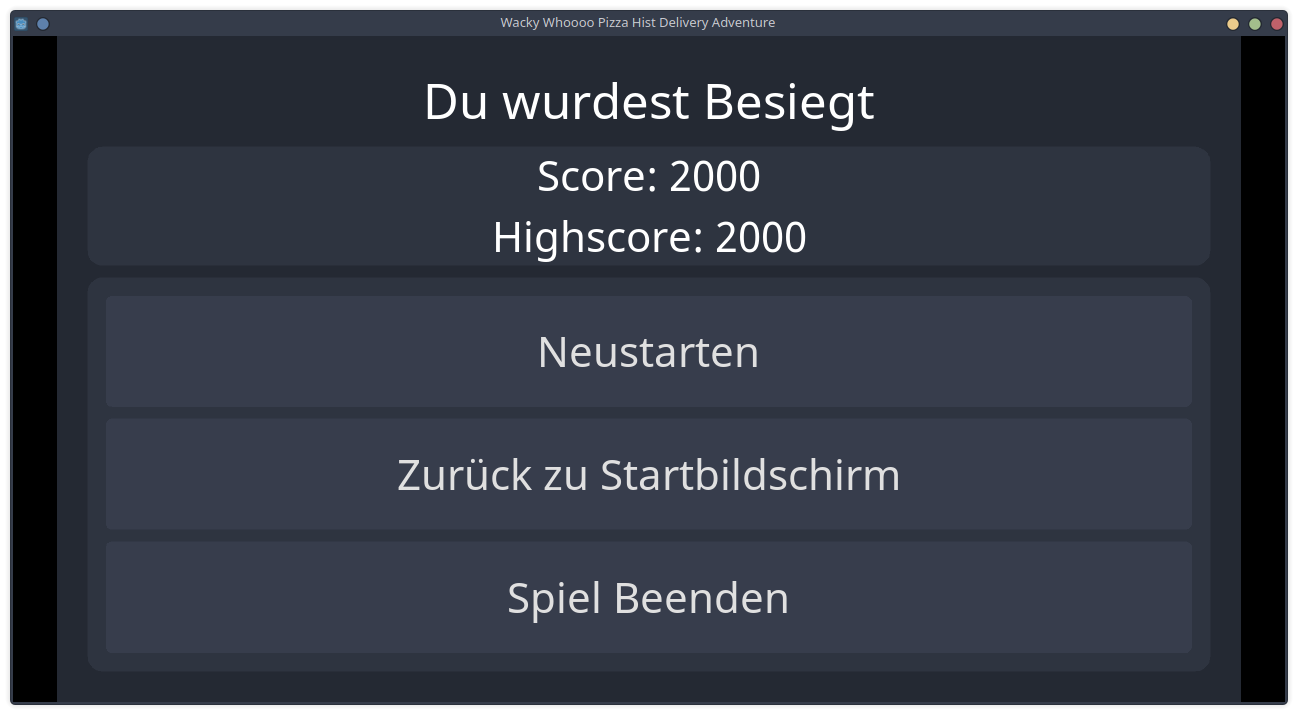
\includegraphics[width=0.8\textwidth]{lose.png}
				\end{center}
				\caption{Niederlagen-Bildschirm}
			\end{figure}

	\section{Fazit}
	
	Die Arbeit an dem Spieleprojekt hat mir viel Spaß bereitet. Des Weiteren habe ich auch einiges über die Godot Engine und generelle Spieleentwicklung gelernt. Ich bin mit meiner Entscheidung die Godot Engine anstatt Greenfoot zu nehmen sehr zufrieden, da ich mit dem Wissen über die Godot Engine und der generellen Spieleentwicklung, welches ich mir für dieses Projekt aneignen musste, das Gefühl habe, in der Lage zu sein ein komplexeres Spiel zu entwickeln. Das Programmieren in der Godot Engine war aufgrund der eigenen Sprache etwas gewöhnungsbedürftig, jedoch hatte man diese aufgrund ihrer Ähnlichkeit zu Python schnell gelernt. Danach war das Programmieren des Spiels relativ angenehm. Besonders hat mir auch gefallen, dass ich in der Lage war das gesamte Spiel mit FOSS Software zu entwickeln. Der einzige Aspekt, welcher mir als äußerst nervig und schmerzvoll im Gedächtnis geblieben ist, war das Zeichnen der Grafiken. Wie schon oben angesprochen hatte ich eigentlich vor noch mehr Features in das Spiel einzubauen. Jedoch habe ich leider nach Version 1.0 ziemlich die Lust an diesem Projekt verloren, weshalb ich mir nicht vorstellen könnte später mal ein Spiel aus eigenem Willen zu entwickeln.
	
	
\end{document}
